\section{Problemstellung}

%----------------------------------------------------------------------%SLIDE -
\begin{frame}
    \frametitle{Problemstellung}
    \begin{itemize}
        \item
            Unser Ziel ist es, neuronale Netzwerke zu trainieren, so dass diese
            uns im Go schlagen können.

        \item Zwischenziel / Alternative:
            Können wir neuronale Netze so trainieren, so dass sie besser als
            zufällig erzeugte Netze spielen?
    \end{itemize}

    \hfill \\
    \hfill \\
    TODO: Ziele besser verkaufen
\end{frame}
%----------------------------------------------------------------------%SLIDE -

%----------------------------------------------------------------------%SLIDE -
\begin{frame}
    \frametitle{Go}
    \begin{columns}
        \column{0.5\textwidth}
        \begin{itemize}
            \item Asiatisches Brettspiel
            \item Wird auf Brettern mit $19 \times 19$ Knoten gespielt.
            \item Ziel: Gebiet einkreisen und gegnerische Steine schlagen
            \item Spielende: wenn beide Spieler passen
        \end{itemize}
        \column{0.5\textwidth}
        \begin{figure}
            \centering
            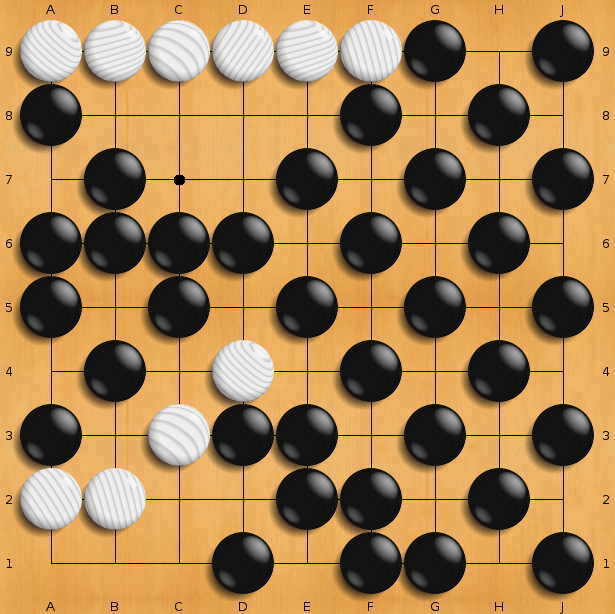
\includegraphics[scale=0.25]{content/img/go_board}
            \caption{generated with qGo}
        \end{figure}
    \end{columns}
\end{frame}
%----------------------------------------------------------------------%SLIDE -

%----------------------------------------------------------------------%SLIDE -
\begin{frame}
    \frametitle{Neuronale Netzwerke}
    \begin{itemize}
        \item Besteht aus mehreren Schichten (layer)
        \item Layer bestehen aus Neuronen
        \item Neuronen benachbarter layer sind alle untereinander verbunden
    \end{itemize}
    \begin{figure}
        TODO: Graphik (möglichst unter CC / selbst erstellt)
        \caption{Schema eines neuronalen Netzwerks}
    \end{figure}
\end{frame}
%----------------------------------------------------------------------%SLIDE -
